\documentclass[12pt]{report}
\usepackage{microtype}
\usepackage[utf8]{inputenc}
\usepackage[english]{babel}
\usepackage{hyperref}
\usepackage{graphicx}
\usepackage{float}
\usepackage{indentfirst}
\usepackage{url}
\usepackage[margin=2cm]{geometry}
\usepackage{titling}
\usepackage{subfigure}
\date{\today}
\title{\Large Semi-Structured Data: \\ XML, XSD, DTD, XPath and XQuery}
\begin{document}
\begin{titlepage}
    \centering
    \vspace*{0.5cm}
    
\includegraphics[scale=0.2]{university-logo.png}\\[1.0cm]	
    \textsc{\LARGE Hassiba Benbouali University}\\[2.0cm]	
	\textsc{\Large Assignment Report}\\[0.5cm]				
	\rule{\linewidth}{0.2mm} \\[0.4cm]
	{\huge \bfseries \thetitle \\[0.4cm] }
	\rule{\linewidth}{0.2mm} \\[1.5cm]
	
	\begin{minipage}{0.4\textwidth}
		\begin{flushleft} \large
			\emph{Authors:}\\
			Abdelhalim Esselami \\
			Abdelkadir Cheklal
		\end{flushleft}
	\end{minipage}~
	\begin{minipage}{0.4\textwidth}
		\begin{flushright} \large
			\emph{Supervisor:} \\
			Boudabous Sofiane							
		\end{flushright}
	\end{minipage}\\[2cm]
	
	{\large \thedate}\\[2cm]
	
	\vfill
\end{titlepage}

\newpage

\tableofcontents
\listoffigures
\newpage
\section{Introduction}
In this report, we will discuss the assignment on "Données Semi-Structurées" and the steps involved in completing it. The assignment involved working with XML data, creating a DTD, developing an XML schema, implementing XSLT and CSS for styling, executing XPath and XQuery queries, and transforming XML to HTML. We will provide an overview of each step and present the solutions implemented.

\section{XML Data}
We started by collecting data related to a tourist trip in the Hautes-Alpes region. The data included information about the guide, the locations, and the itineraries. We organized this data into an XML file named \texttt{trip\_hautes\_alpes.xml}.
\begin{figure}[htbp]
	\centering
	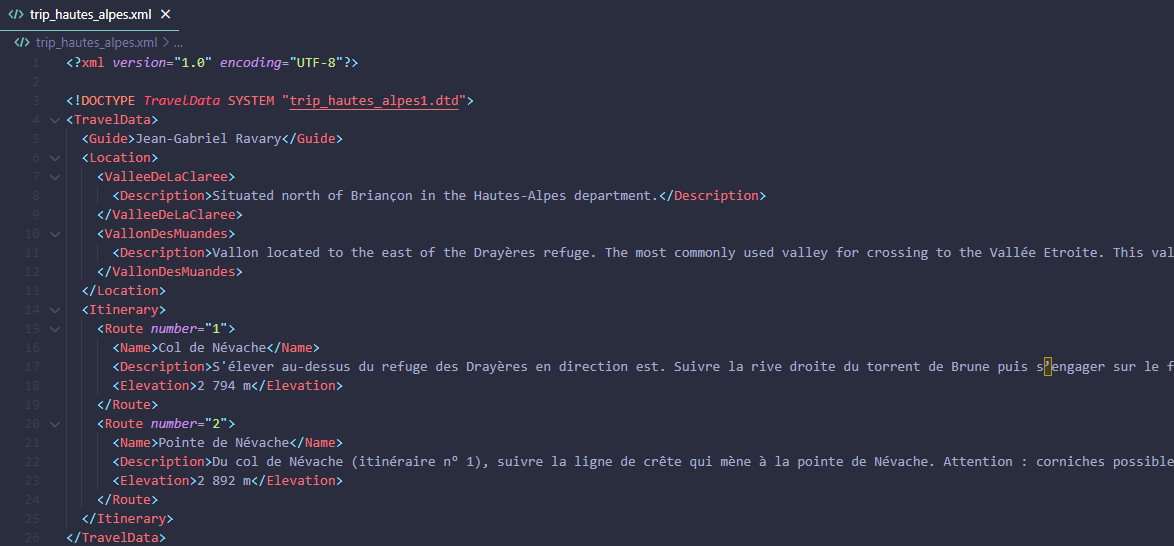
\includegraphics[width=1.0\textwidth]{xml.png}
	\caption{Screenshot of the XML file}
	\label{fig:screenshot}
  \end{figure}
\section{DTD}
To define the structure and constraints of the XML data, we created a Document Type Definition (DTD) file named \texttt{trip\_hautes\_alpes.dtd}. The DTD specified the element structure, allowed content, and attribute declarations.
The DTD (Document Type Definition) file defines the structure and constraints of the XML document for the trip to Hautes-Alpes. It specifies the elements, attributes, and their relationships allowed in the document.

\medskip The DTD consists of the following declarations:
\begin{itemize}
	

\item  \textbf{\textbf{TravelData:}} The root element representing the travel data.
\item  \textbf{Guide:} Element for specifying the guide's name.
\item  \textbf{Location:} Element for describing the various locations.
\item  \textbf{ValleeDeLaClaree:} Element for providing details about Vallee de la Claree.
\item  \textbf{VallonDesMuandes:} Element for providing details about Vallon des Muandes.
\item  \textbf{Itinerary:} Element for defining the travel itineraries.
\item  \textbf{Route:} Element representing an individual travel route.
\item  \textbf{Name:} Element for specifying the name of a route.
\item  \textbf{Description:} Element for describing the details of a route.
\item  \textbf{Elevation:} Element for specifying the elevation of a route.
\item  \textbf{Route number:} Attribute for assigning a number to a route.
\end{itemize}
The DTD enforces the structure and content rules for the XML document, ensuring it conforms to the defined schema.

This DTD file is used to validate and ensure the integrity of the XML data for the trip to Hautes-Alpes.
\begin{figure}[htbp]
	\centering
	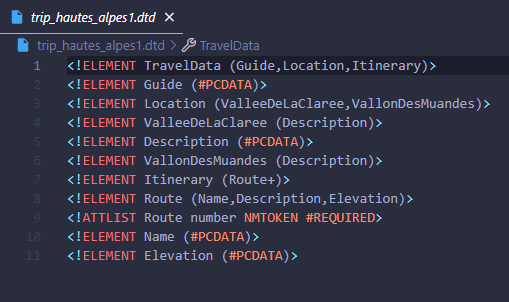
\includegraphics[width=1.0\textwidth]{dtd.png}
	\caption{Screenshot of the DTD file}
	\label{fig:screenshot1}
  \end{figure}
  \clearpage
\section{XML Schema}

Next, we developed an XML Schema Definition (XSD) file named \texttt{trip\_hautes\_alpes.xsd}. 
The XML schema provided a more robust and flexible way to define the structure and constraints of the XML data compared to DTD.

\bigskip Here are some screenshots:

\begin{figure}[htbp]
	\centering
	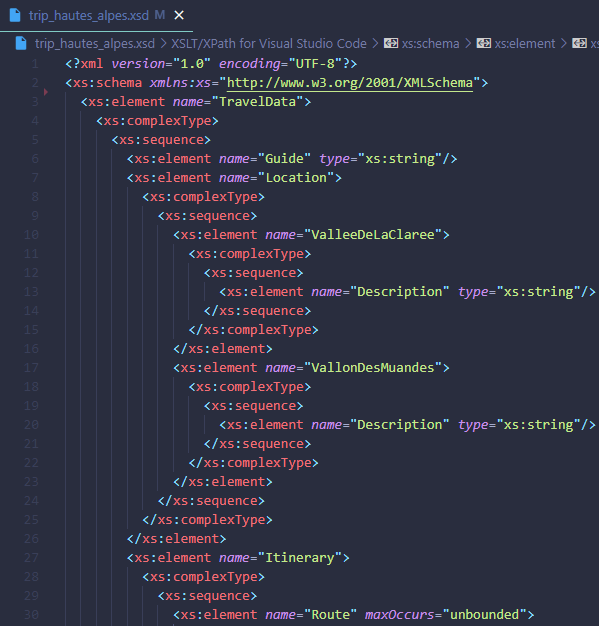
\includegraphics[width=0.7\textwidth]{xsd.png}
	\caption{Screenshot of the XSD file}
	\label{fig:screenshot2}
  \end{figure}
  \begin{figure}[htbp]
	\centering
	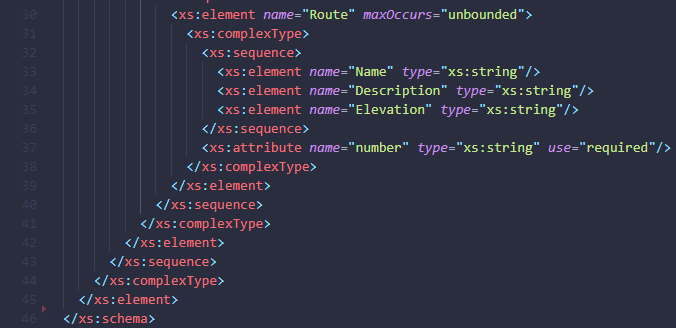
\includegraphics[width=1.0\textwidth]{xsd2.png}
	\caption{Screenshot of the XSD file}
	\label{fig:screenshot3}
  \end{figure}
  \begin{figure}[htbp]
	\centering
	\subfigure[First Screenshot]{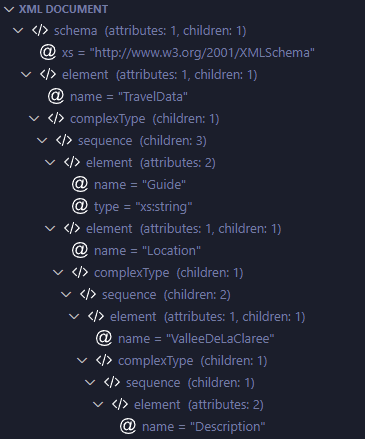
\includegraphics[width=0.3\textwidth]{schema1.png}}
	\hfill
	\subfigure[Second Screenshot]{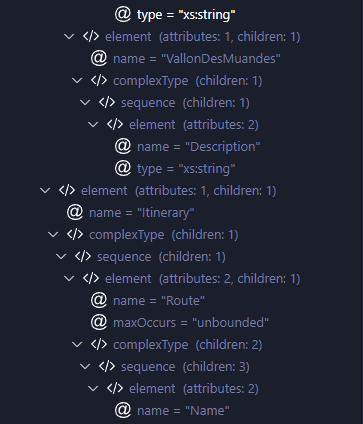
\includegraphics[width=0.3\textwidth]{schema2.png}}
	\hfill
	\subfigure[Third Screenshot]{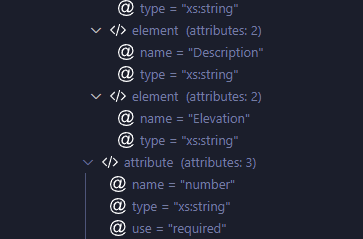
\includegraphics[width=0.3\textwidth]{schema3.png}}
	\caption{The Schema}
	\label{fig:multiple-screenshots}
  \end{figure}
\newpage 
\section{XSLT and CSS}
To transform the XML data into HTML and apply styling, we created an XSLT file named \texttt{transform.xsl}. The XSLT file defined templates and rules to transform the XML elements into HTML elements. We also developed a CSS file named \texttt{style.css} to apply styles and layout to the HTML output.
\begin{figure}[htbp]
	\centering
	\subfigure[First Screenshot]{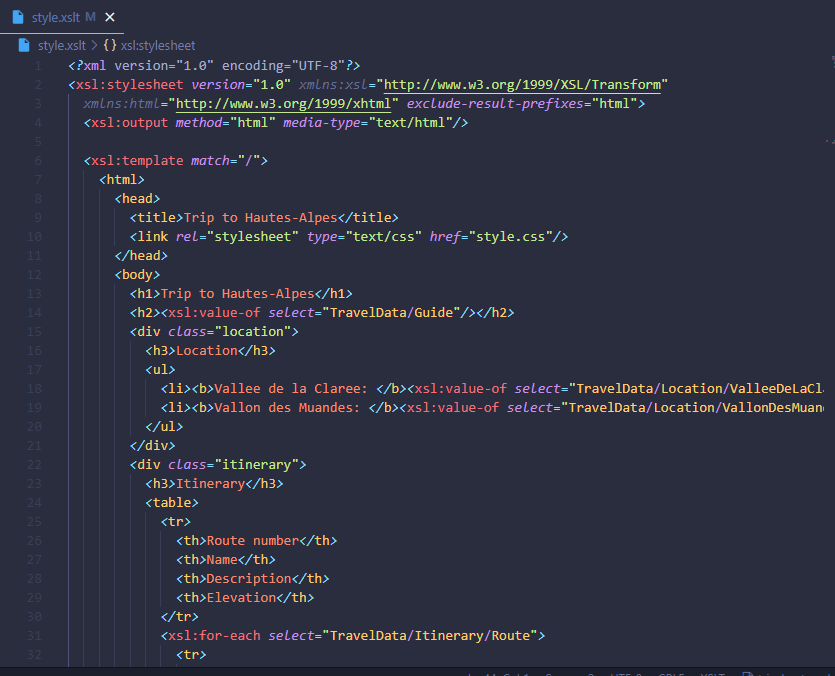
\includegraphics[width=0.8\textwidth]{xslt.png}}
	\subfigure[Second Screenshot]{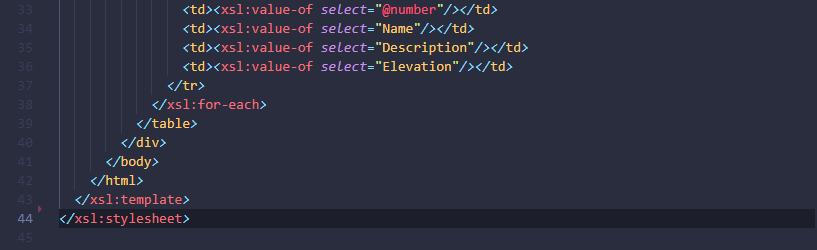
\includegraphics[width=0.8\textwidth]{xslt2.png}}
	\caption{XSLT file}
	\label{fig:multiple-screenshots2}
  \end{figure}
  \begin{figure}[htbp]
	\centering
	\subfigure[First Screenshot]{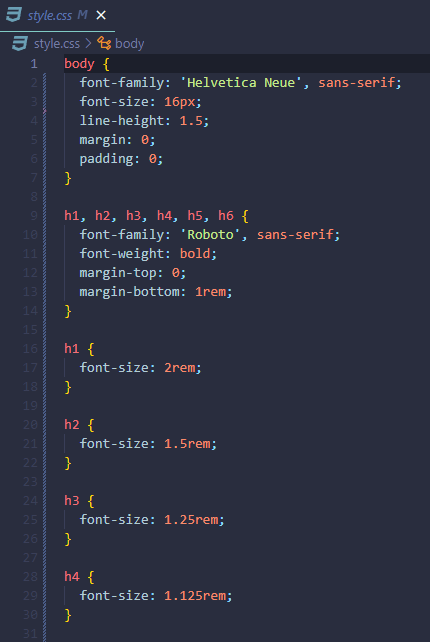
\includegraphics[width=0.3\textwidth]{css.png}}
	\subfigure[Second Screenshot]{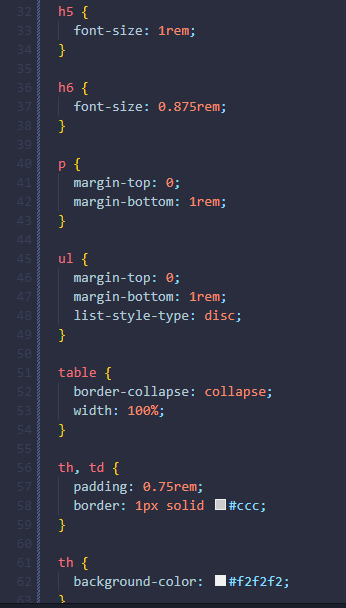
\includegraphics[width=0.3\textwidth]{css2.png}}
	\subfigure[Second Screenshot]{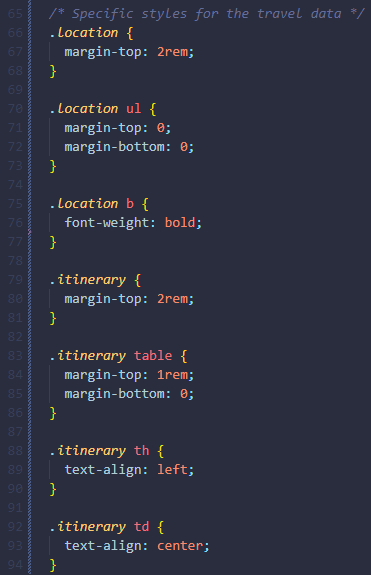
\includegraphics[width=0.3\textwidth]{css3.png}}
	\caption{CSS file}
	\label{fig:multiple-screenshots3}
  \end{figure}  
\section{XPath and XQuery}
Using XPath and XQuery, we performed queries on the XML data. With XPath, we retrieved all the itineraries using the expression \texttt{/TravelData/Itinerary/Route}. With XQuery, we obtained the names of the tour guides using the query \texttt{for \$guide in /TravelData/Guide return \$guide}.
\begin{figure}[htbp]
	\centering
	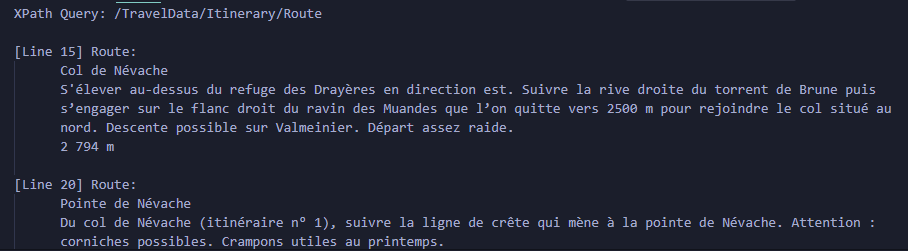
\includegraphics[width=1.0\textwidth]{xpath.png}
	\caption{XPath Output}
	\label{fig:multiple-screenshots4}
  \end{figure} 
 

\section{XML to HTML Transformation}
Finally, we executed the XSLT transformation to convert the XML data to HTML using the Saxon XSLT processor. The output HTML file named \texttt{output.html} displayed the trip information with the applied styles defined in the CSS file.

\medskip The command used :
\begin{verbatim}
	xsltproc -o output.html style.xslt trip_hautes_alpes.xml
\end{verbatim}

\begin{figure}[htbp]
	\centering
	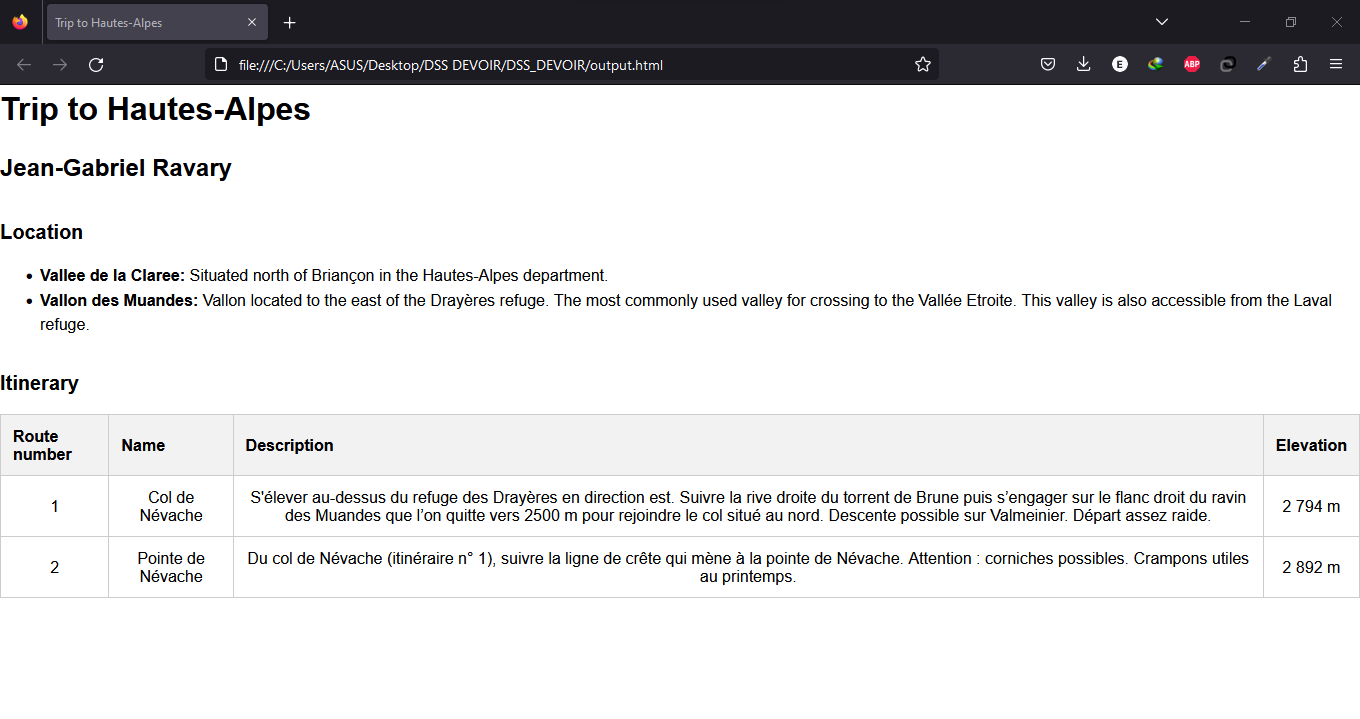
\includegraphics[width=1.0\textwidth]{output.png}
	\caption{XPath Output}
	\label{fig:multiple-screenshots5}
  \end{figure} 
  \newpage
\section{Conclusion}
In conclusion, the assignment on "Données Semi-Structurées" involved working with XML data, creating a DTD, developing an XML schema, implementing XSLT and CSS for styling, executing XPath and XQuery queries, and transforming XML to HTML. By following the provided instructions and utilizing the appropriate tools, we successfully completed the assignment and obtained the desired results.
XML (eXtensible Markup Language) has proven to be a valuable tool for structuring and organizing data in a hierarchical and self-descriptive format. Throughout this assignment, we explored the use of XML for representing travel data related to a trip in the Hautes-Alpes region. XML's flexibility allows us to define custom elements and attributes tailored to our specific needs, such as defining the guide, locations, and itineraries.

By adhering to a defined DTD and XML schema, we ensure the integrity and consistency of the data. The DTD serves as a blueprint for the structure of the XML document, while the XML schema provides a more robust validation mechanism with data types, constraints, and more.

Additionally, we leveraged XPath and XQuery to query and extract specific information from the XML data. XPath provided a concise and powerful syntax for navigating the XML hierarchy and selecting elements based on criteria. XQuery allowed us to perform more complex queries, such as retrieving the names of the tourist guides.

Overall, XML offers a standardized and versatile approach to storing and exchanging data, making it a widely adopted technology in various domains. Its ability to represent both structured and semi-structured data makes it suitable for a wide range of applications, including data integration, document storage, and web services.

In conclusion, our exploration of XML and its associated technologies has provided valuable insights into the benefits and capabilities of this markup language. As technology continues to evolve, XML remains a fundamental tool for managing and exchanging data in a structured and interoperable manner.
\end{document}